% Autoregression: one factorisation, two computational organisations.
% Training scores every position in a single parallel teacher-forced pass;
% decoding feeds its own sampled tokens back, one step at a time (exposure bias).
\documentclass[border=0pt]{standalone}
\usepackage{amsmath,amssymb}
% Shared visual language for the figures of the book.
% Every figure in this directory loads this file so the chapter reads as one system.
% NOTE: no blank lines are allowed inside \tikzset{...} (a blank line emits \par
% and breaks key scanning).
\NeedsTeXFormat{LaTeX2e}
\ProvidesPackage{figstyle}[2026/10/21 Figure style for Free Energy to LLMs]

\RequirePackage{tikz}
\usetikzlibrary{arrows.meta,positioning,calc,fit,shapes.geometric,shapes.misc,%
  backgrounds,matrix,decorations.pathreplacing,decorations.markings,patterns.meta}

% ---------------------------------------------------------------- palette
% Same values as book/preamble/style.tex, prefixed with F.
\definecolor{FNavy}{HTML}{14324A}
\definecolor{FTeal}{HTML}{0E7490}
\definecolor{FSky}{HTML}{E7F5F8}
\definecolor{FOrange}{HTML}{D97706}
\definecolor{FAmber}{HTML}{FFF3D6}
\definecolor{FInk}{HTML}{1F2937}
\definecolor{FSlate}{HTML}{64748B}
\definecolor{FMist}{HTML}{F5F7FA}
\definecolor{FRose}{HTML}{9F1239}
\definecolor{FRoseMist}{HTML}{FFF1F2}

% ---------------------------------------------------------------- semantics
% Teal   = probability / model / data object
% Orange = training objective, cost, or the quantity moved through the system
% Navy   = neutral structure
% Slate  = secondary label or metadata
% Rose   = failure mode, hazard, masked-out region
\tikzset{
  % Lay figures out in millimetres.  A figure designed 168mm wide is included at
  % \textwidth, so its fonts appear at exactly the size written here.
  every picture/.style={x=1mm,y=1mm,font=\small,line cap=round,line join=round},
  % ---- block styles
  nbase/.style={draw,rounded corners=1.2pt,align=center,inner sep=2.4pt,%
    minimum height=7mm,text=FInk},
  nteal/.style={nbase,draw=FTeal,fill=FSky},
  norange/.style={nbase,draw=FOrange,fill=FAmber},
  nnavy/.style={nbase,draw=FNavy,fill=white},
  nsoft/.style={nbase,draw=FSlate!55,fill=FMist},
  nrose/.style={nbase,draw=FRose,fill=FRoseMist},
  ghost/.style={draw=none,fill=none,align=center,inner sep=1pt},
  plain/.style={draw=none,fill=none,align=center,inner sep=0pt},
  % ---- arrows
  ar/.style={-{Latex[length=1.7mm,width=1.35mm]},draw=FSlate,line width=0.75pt},
  ard/.style={ar,dashed},
  arteal/.style={ar,draw=FTeal},
  arorange/.style={ar,draw=FOrange},
  arrose/.style={ar,draw=FRose},
  thickar/.style={ar,line width=1.2pt},
  % ---- text roles
  ftitle/.style={font=\large\bfseries,text=FNavy,align=center},
  ptitle/.style={font=\small\bfseries,text=FNavy,align=center},
  ptitleo/.style={font=\small\bfseries,text=FOrange,align=center},
  lbl/.style={font=\scriptsize,text=FSlate,align=center,inner sep=1pt},
  lblt/.style={lbl,text=FTeal},
  lblo/.style={lbl,text=FOrange},
  lbln/.style={lbl,text=FNavy},
  lblr/.style={lbl,text=FRose},
  sub/.style={font=\scriptsize,text=FSlate!90,align=center,inner sep=1pt},
  monob/.style={font=\ttfamily\scriptsize,text=FInk,inner sep=1pt},
  mathb/.style={font=\small,text=FInk,inner sep=1pt},
  eqn/.style={font=\scriptsize,inner sep=1.5pt,text=FInk},
  % ---- decorations
  brace/.style={decorate,decoration={brace,amplitude=2.4pt},draw=FSlate,%
    line width=0.6pt},
  bracet/.style={brace,draw=FTeal},
  braceo/.style={brace,draw=FOrange},
  axis/.style={draw=FSlate!55,line width=0.6pt},
  guide/.style={draw=FSlate!45,line width=0.5pt,dashed},
  halolabel/.style={font=\scriptsize,text=FInk,fill=white,fill opacity=0.85,%
    text opacity=1,inner sep=1.4pt,align=center},
}

% Figure title above the drawing, anchored at the figure's top-left.
\newcommand{\figtitle}[2][0]{%
  \node[ftitle,anchor=north west,outer sep=0pt] at (#1,0) {#2};}

% Rounded panel behind a subgroup of nodes.
\newcommand{\figpanel}[3][]{%
  \node[draw=FSlate!35,fill=#3,rounded corners=2pt,inner sep=2.6mm,#1] {#2};}

\endinput

\begin{document}
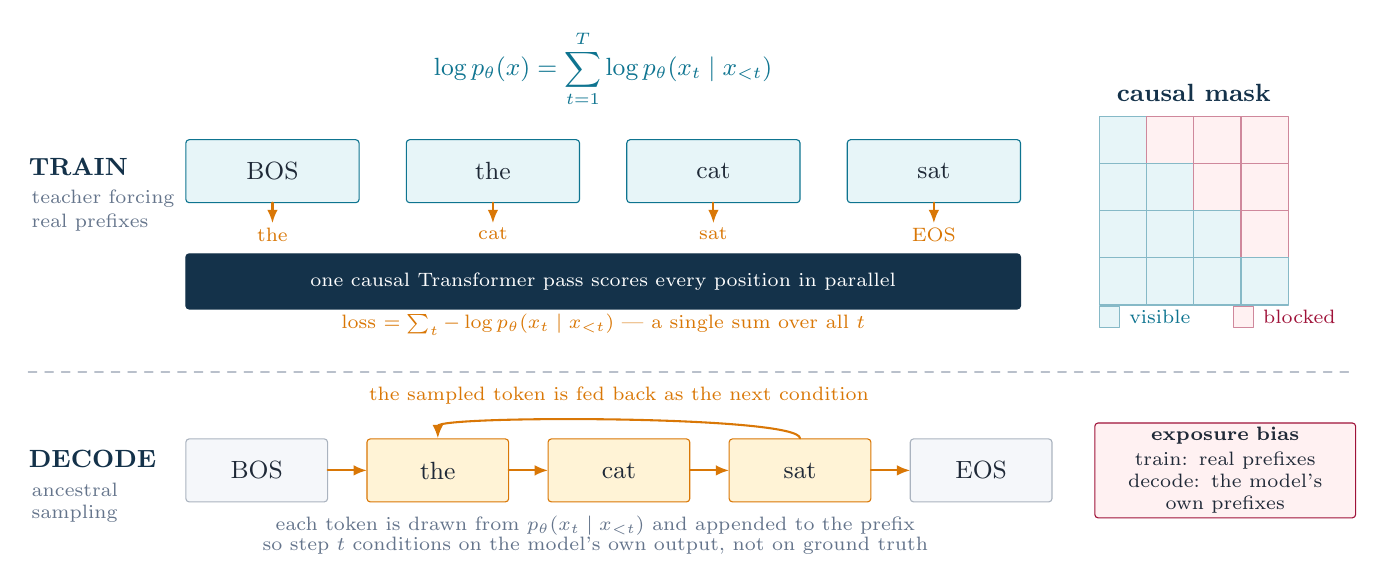
\begin{tikzpicture}
\node[mathb,text=FTeal] at (73,68) {$\displaystyle \log p_\theta(x)=\sum_{t=1}^{T}\log p_\theta(x_t\mid x_{<t})$};
\node[plain,anchor=west,font=\small\bfseries,text=FNavy] at (0,55.5) {TRAIN};
\node[lbl,anchor=west] at (0,51.5) {teacher forcing};
\node[lbl,anchor=west] at (0,48.5) {real prefixes};
\node[nteal,minimum width=22mm,minimum height=8mm] (t0) at (31,55) {BOS};
\node[nteal,minimum width=22mm,minimum height=8mm] (t1) at (59,55) {the};
\node[nteal,minimum width=22mm,minimum height=8mm] (t2) at (87,55) {cat};
\node[nteal,minimum width=22mm,minimum height=8mm] (t3) at (115,55) {sat};
\foreach \i/\tok in {0/the,1/cat,2/sat,3/EOS}{
  \draw[arorange] (31+28*\i,51) -- (31+28*\i,48.4);
  \node[lblo,anchor=north] at (31+28*\i,48.2) {\tok};}
\node[fill=FNavy,draw=FNavy,rounded corners=1.2pt,minimum width=106mm,minimum height=7mm,text=white,font=\scriptsize,inner sep=1pt] at (73,41) {one causal Transformer pass scores every position in parallel};
\node[lblo] at (73,35.5) {loss $=\sum_{t}-\log p_\theta(x_t\mid x_{<t})$ — a single sum over all $t$};
\foreach \t in {0,1,2,3}{
  \foreach \j in {0,1,2,3}{
    \ifnum\j>\t
      \fill[FRoseMist] (136+6*\j,56-6*\t) rectangle ++(6,6);
      \draw[FRose!50,line width=0.4pt] (136+6*\j,56-6*\t) rectangle ++(6,6);
    \else
      \fill[FSky] (136+6*\j,56-6*\t) rectangle ++(6,6);
      \draw[FTeal!50,line width=0.4pt] (136+6*\j,56-6*\t) rectangle ++(6,6);
    \fi}}
\node[ptitle] at (148,65) {causal mask};
\fill[FSky] (136,35.2) rectangle ++(2.6,2.6);
\draw[FTeal!50,line width=0.4pt] (136,35.2) rectangle ++(2.6,2.6);
\node[lblt,anchor=west] at (139.4,36.5) {visible};
\fill[FRoseMist] (153,35.2) rectangle ++(2.6,2.6);
\draw[FRose!50,line width=0.4pt] (153,35.2) rectangle ++(2.6,2.6);
\node[lblr,anchor=west] at (156.4,36.5) {blocked};
\draw[guide] (0,29.5) -- (168,29.5);
\node[plain,anchor=west,font=\small\bfseries,text=FNavy] at (0,18.5) {DECODE};
\node[lbl,anchor=west] at (0,14.5) {ancestral};
\node[lbl,anchor=west] at (0,11.5) {sampling};
\node[nsoft,minimum width=18mm,minimum height=8mm] (d0) at (29,17) {BOS};
\node[norange,minimum width=18mm,minimum height=8mm] (d1) at (52,17) {the};
\node[norange,minimum width=18mm,minimum height=8mm] (d2) at (75,17) {cat};
\node[norange,minimum width=18mm,minimum height=8mm] (d3) at (98,17) {sat};
\node[nsoft,minimum width=18mm,minimum height=8mm] (d4) at (121,17) {EOS};
\draw[arorange] (38,17) -- (43,17);
\draw[arorange] (61,17) -- (66,17);
\draw[arorange] (84,17) -- (89,17);
\draw[arorange] (107,17) -- (112,17);
\draw[arorange] (d3.north) .. controls (98,24) and (52,24) .. (d1.north);
\node[lblo] at (75,26.5) {the sampled token is fed back as the next condition};
\node[lbl] at (72,10) {each token is drawn from $p_\theta(x_t\mid x_{<t})$ and appended to the prefix};
\node[lbl] at (72,7.4) {so step $t$ conditions on the model's own output, not on ground truth};
\node[nrose,text width=32mm,inner sep=1.6pt,align=center,font=\scriptsize] at (152,17) {\textbf{exposure bias}\\[0.3mm] train: real prefixes\\ decode: the model's\\ own prefixes};
\end{tikzpicture}
\end{document}
